\documentclass{article}

\usepackage{tikz,pgfplots}
\usepackage{pgfplotstable}
\usepgfplotslibrary{fillbetween}

\pgfplotsset{compat=1.12} 

\begin{document}

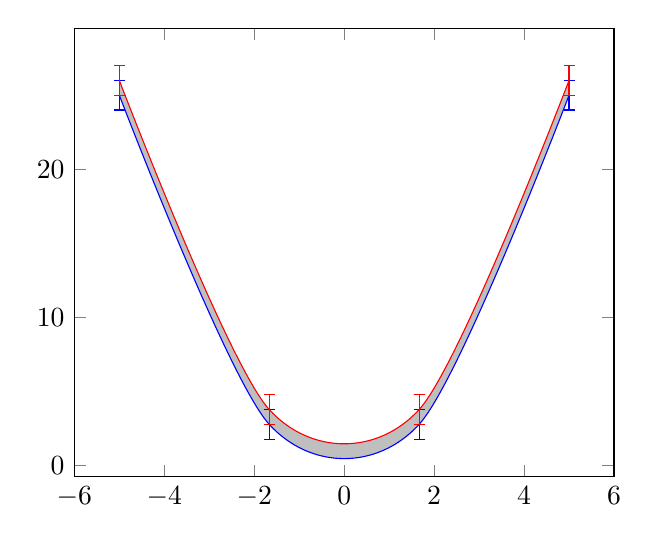
\begin{tikzpicture}
\begin{axis}[ 
    error bars/y dir=both,
    error bars/y fixed=1, 
	samples=4,
    ]

    \addplot[blue,name path=A,smooth] {x^2};
    \addplot[red,name path=B,smooth]  {x^2+1};
    \addplot[gray!50] fill between[of=A and B];

\end{axis}
\end{tikzpicture} 

\end{document}
